\documentclass[conference]{IEEEtran}
\usepackage[T1]{fontenc}
\usepackage{amsmath,amssymb}
\usepackage{graphicx}
\usepackage{booktabs}
\usepackage{cite}
\usepackage[hidelinks]{hyperref}
\usepackage{float}

% Numbers are from robotnik_arm/experiments/ablation/results/rel_study/.
% Budget: six IEEE pages including references; the contribution statement
% may occupy a separate seventh page.
% Scope: one-ball behaviour cloning with a flat network.

\title{Learning to Catch with Behaviour Cloning:\\
Accuracy and Closed-Loop Failure Analysis}
\author{\IEEEauthorblockN{William Boyd, Nick Wright, Yiyan Wang}
\IEEEauthorblockA{University College London\\London, United Kingdom}}

\begin{document}
\maketitle

\begin{abstract}
A flat behaviour-cloning policy imitates a scripted controller that intercepts one ball with a mobile manipulator. Every model, including the $10\,\mathrm{Hz}$ baseline, uses the same base-frame ball features. The baseline's commands are analysed before a pre-registered sweep of policy rate, history, prediction horizon and execution window. Faster rates lower the miss, as that analysis indicated, and the ranking rule selects $25\,\mathrm{Hz}$, predicting $2\,\mathrm{s}$ and executing $1\,\mathrm{s}$, with no history: $3.2\%$ of episodes finish within $10\,\mathrm{mm}$ and the mean miss is $59\,\mathrm{mm}$, against $0.7\%$ and $113\,\mathrm{mm}$ at $10\,\mathrm{Hz}$. A $50\,\mathrm{Hz}$ policy has a higher catch rate, but the seed intervals overlap and its miss is not lower. Retraining the winner on high-amplitude command noise matched to its own error raises the mean miss to $90\,\mathrm{mm}$. Adding demonstrations that park the base off the expert's point lowers it to $28\,\mathrm{mm}$, by correcting sideways parking error. The along-track correction does not improve.
\end{abstract}

\begin{IEEEkeywords}
Imitation learning, mobile manipulation, robotic catching, evaluation
\end{IEEEkeywords}

\section{Introduction}
\subsection{Problem and Scope}
We extend the original fixed-target reaching task to moving target interception ("ball-catching"), still using the robot with the mobile base and seven-joint arm. Behaviour cloning is used to train a neural network to imitate the commands generated by the expert controller~\cite{pomerleau1991}. To catch a moving ball, a robot can move its hand to different points along the ball’s trajectory, changing the problem from reaching one fixed target to choosing between several valid positions. 

A model may closely match the expert’s recorded commands but still miss the ball when controlling the robot, because each small mistake changes the robot’s position and affects the movements that follow~\cite{ross2011}. We therefore let the learner operate the simulated robot from its starting state until a catch or timeout, measuring the distance between the hand and the ball and how this relates to errors in the base position. These tests use simulated state measurements and ball paths that the expert can catch, with a catch defined as the hand coming to rest within a set distance of the ball, without requiring a grab with the finger joints.

\subsection{Research Question and Contributions}
We investigate how policy rate, observation history, prediction horizon and execution window affect ball-catching accuracy. The study analyses a $10\,\mathrm{Hz}$ baseline first, then varies one of those factors at a time. The winning configuration is retrained on two further demonstration sets: high-amplitude command noise, and deliberate off-target parking. Unsuccessful runs are kept, so the comparison can show where the error remains.


\section{Methodology}
% Approx. 1.25 pages, including a compact training/configuration table.
\subsection{Simulation Environment and Task Definition}
The simulated robot has a skid-steer base, a seven-degree-of-freedom Kinova arm and a passive hand, with PyBullet providing the physics simulation~\cite{pybullet} and Pinocchio calculating the robot's kinematics and rigid-body dynamics~\cite{pinocchio}. The simulation advances in $1\,\mathrm{ms}$ steps within a workspace measuring $5\times5\,\mathrm{m}$ horizontally, centred on the robot’s initial base position, with height limits of $0.07$–$1.30\,\mathrm{m}$. Each ball follows a seeded parabolic path between randomly sampled points on opposite vertical faces of the workspace. Its peak is sampled between $0.5$ and $1.5,\mathrm{m}$ above the roof, ensuring that it leaves the workspace and re-enters before reaching the opposite face. Paths are retained only if the expert planner finds a feasible interception before the endpoint.
\begin{figure}[H]
    \centering
    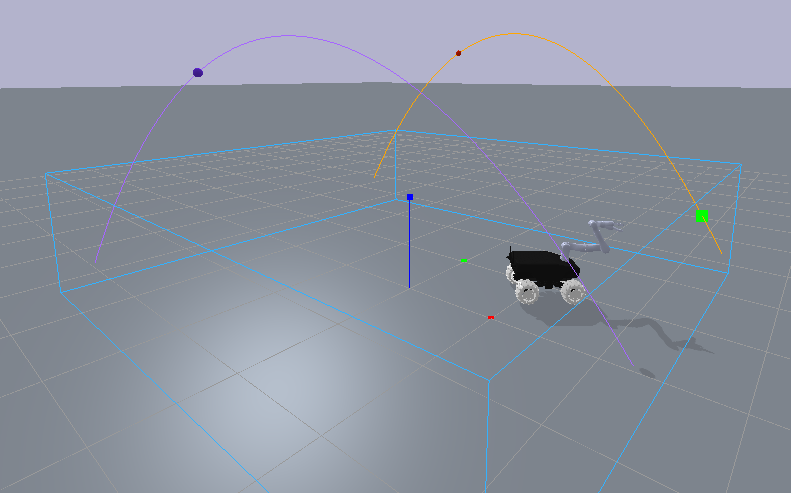
\includegraphics[width=0.75\columnwidth]{image.png}
    \caption{Simulated single-ball catching task, showing the
    mobile robot, workspace boundaries and target interception point}
    \label{fig:image}
\end{figure}
\subsection{Expert and Demonstration Generation}
We extend the provided fixed-target expert with an interception planner that estimates the ball's velocity and acceleration from three position observations. It searches future points along the predicted path in $0.1\,\mathrm{s}$ increments, selecting the earliest feasible interception after re-entry into the workspace and a base position and heading from which the arm can reach it. Feasibility accounts for base travel, turning and arm movement, with extra time for settling. The existing base and arm controllers then move towards these planned goals, with replanning if the interception is missed by more than $1\,\mathrm{s}$. The model is trained to predict the wheel and arm commands produced by the expert.


\subsection{Dataset and Later Demonstration Extensions}
The baseline and the factor sweep use 1,000 demonstrations, one per training scene, resampled to a $50\,\mathrm{Hz}$ grid. Odd-indexed demonstrations already contain a small perturbation added when the set was collected~\cite{laskey2017}. It is Gaussian noise on the applied wheel and arm torques, with standard deviations $0.08$ and $0.2\,\mathrm{N{\cdot}m}$, clipped at three standard deviations and held for $50\,\mathrm{ms}$. The stored label is the clean expert command. This is not the high-amplitude comparison below. Master seed 2026 generates the 1,000 training scene seeds and 200 separate evaluation scene seeds. Evaluation scenes use the same generation rules and parameter distributions.

After a winner is selected, that same configuration is trained twice more. Each added set contains 1,000 episodes on the training seeds. One set perturbs the expert's executed commands with high-amplitude noise matched to the winner's own command error, and stores the clean expert command as the label. The other shifts the expert's parking position and leaves the commands clean. Shifts along and across the route are drawn from zero-mean Gaussians with standard deviations of $20$ and $50\,\mathrm{mm}$, and the shift vector is limited to $150\,\mathrm{mm}$. The two extensions therefore add the same scenes and the same number of episodes. They differ in what is perturbed.

\begin{table}[t]
\centering
\caption{Demonstration sets used in this study. The extensions reuse the training scene seeds.}
\label{tab:datasets}
\begin{tabular}{lcc}
\toprule
Set & Episodes & What is added \\
\midrule
Ablation & 1,000 & Low-amplitude torque noise on odd episodes \\
Command noise & 2,000 & 1,000 high-amplitude DART episodes \\
Parking offset & 2,000 & 1,000 shifted parking positions \\
\bottomrule
\end{tabular}
\end{table}

\subsection{Observation Representation and Temporal Context}
Each raw observation contains 42 values: time; ball position, velocity and acceleration; base position; heading as a sine and cosine; base linear and angular velocity; seven arm joint positions and velocities; four wheel velocities; and end-effector position. Ball velocity and acceleration are estimated from the last three $1\,\mathrm{ms}$ samples, which is the estimate the expert uses. The model receives these state measurements rather than camera images.

Every model in this study, including the baseline, appends twelve base-frame features to that 42-value observation. Ball position is written relative to the base origin. Ball velocity, ball acceleration, and the ball's displacement from the hand are the corresponding world vectors rotated into the robot's forward, sideways and vertical axes. The network is a flat multilayer perceptron over this vector. It has no separate ball encoder.

The baseline conditions on the current frame only. History is one of the factors varied later: a stack of frames covering $0.5\,\mathrm{s}$ or $2\,\mathrm{s}$, or a recurrent summary over $2\,\mathrm{s}$. The ranked winner uses the current frame only.

\subsection{Policy Architecture and Action Chunking}
The network is three fully connected layers of width 512, each followed by a ReLU, and a linear head. With no history the input is the current 54-value frame. A stack flattens the frames. The GRU variant, hidden size 128, appends its final state to the current frame. The head emits a chunk of 18-value commands, one per future label step: four wheel velocities, seven arm joint references and seven joint-velocity references. Joint references are labelled relative to the arm position at the query, and at execution they are added back to that same position and held while the chunk runs. There is no learned ball encoder.

The simulation keeps its $1\,\mathrm{ms}$ step. Between policy queries the low-level loop holds the latest command. Wheel torque is $-30$ times the wheel-speed error. The arm uses the expert's gravity-compensated proportional-derivative law, with the joint reference clipped to a limited lead from the measured angle. When the policy rate changes, the predicted and executed durations stay fixed in seconds, so a faster rate produces more steps. The baseline predicts $2\,\mathrm{s}$ and executes $1\,\mathrm{s}$.
\subsection{Training Configuration}
Inputs are standardised using statistics from the training observations, while action targets use statistics from up to 50,000 sampled training windows, with standard deviations floored at $10^{-3}$ and normalised inputs clipped to $[-10,10]$. Training minimises mean squared error over the normalised action sequence, repeating the first observation where a history window extends before an episode and the last command where a target sequence extends beyond its end. The shared settings are AdamW with learning rate $10^{-3}$, weight decay $10^{-4}$, batch size 1,024 and 20,000 steps, three training seeds, and the 200 evaluation scenes. In the one-factor sweeps, rate, history, prediction horizon and execution window are changed one at a time against the $10\,\mathrm{Hz}$ baseline (predict $2\,\mathrm{s}$, execute $1\,\mathrm{s}$, no history). A combination stage is the only place those choices vary together. The winner is the configuration with the higher mean catch rate at $10\,\mathrm{mm}$; if the seed intervals overlap, the lower mean miss is kept. The learning rate warms up linearly over 500 steps and then follows a cosine down to one percent of its peak. There is no validation split and no early stopping.

\begin{table}[t]
\centering
\caption{One-factor levels. Unlisted settings stay at the $10\,\mathrm{Hz}$ baseline: predict $2\,\mathrm{s}$, execute $1\,\mathrm{s}$, current frame only.}
\label{tab:factors}
\begin{tabular}{ll}
\toprule
Factor & Levels other than the baseline \\
\midrule
Policy rate & 5, 25 and $50\,\mathrm{Hz}$ \\
History & Stacks of $0.5\,\mathrm{s}$ and $2\,\mathrm{s}$; GRU over $2\,\mathrm{s}$ \\
Prediction horizon & $1\,\mathrm{s}$ and $5\,\mathrm{s}$, execution held at $1\,\mathrm{s}$ \\
Execution window & $0.5\,\mathrm{s}$, prediction held at $2\,\mathrm{s}$ \\
Short chunk & Predict $0.5\,\mathrm{s}$ (five steps); execute three steps ($0.3\,\mathrm{s}$) or one ($0.1\,\mathrm{s}$) \\
\bottomrule
\end{tabular}
\end{table}

Rate, history and timing are scored as three families. The combination stage crosses the top two levels of the two families that beat the baseline, and adds the single best level of every family that moved. If none beat the baseline, the baseline remains the winner.

\section{Evaluation Protocol}
\label{sec:eval}
For each model, the learned controller runs the simulated robot from its initial state until a catch or timeout, using the same scene seeds so that models face the same ball paths. We measure distance only while the ball is inside the cuboid after previously leaving it; denoting these observed times by $\mathcal{V}_i$, the miss distance for episode $i$ is
\begin{equation}
 d_i=\min_{t\in\mathcal{V}_i}\|\mathbf{p}_{\mathrm{EE},i}(t)-\mathbf{p}_{\mathrm{ball},i}(t)\|_2.
\end{equation}
A catch can count before base navigation is complete, provided the ball meets the capture conditions above. The episode ends $0.1\,\mathrm{s}$ after the hand first comes within $10\,\mathrm{mm}$ of the ball, or at the trajectory duration plus $1\,\mathrm{s}$, whichever occurs first, so the minimum distance covers only the valid times observed before that stopping point. Episodes without a valid capture sample must count as failures and be identified separately when reporting distances.

\subsection{Closed-Loop Episodes and Capture Conditions}
A distance counts only after the ball has left the workspace and come back inside it. The catch radius used for the ranking is $10\,\mathrm{mm}$. Coming within that radius is not a grasp: the fingers stay at a fixed angle. The same 200 evaluation scenes are used for every model. They are the development benchmark for this study, not a fresh final test held out from every design choice.

\subsection{Accuracy and Statistical Uncertainty}
The catch rate on $N$ scenes is
\begin{equation}
\hat{c}=\frac{1}{N}\sum_{i=1}^{N}\mathbf{1}\{d_i<10\,\mathrm{mm}\}.
\end{equation}
The mean and median miss use the same per-scene distances. An episode with no sample inside the capture window is a failure and is reported separately rather than given a finite distance. In this study every evaluation episode produced a finite miss. Each configuration is trained three times. Tables give the mean across those seeds and the sample standard deviation, with the usual $n-1$ divisor. That is the spread used by the ranking rule. The median, where quoted, pools the episodes of the three seeds. Scene-to-scene variation is the distribution in Fig.~\ref{fig:miss}. Because every model faces the same scenes, a difference on those scenes is paired, but the tables do not replace that pairing with a per-scene significance test.

\subsection{Diagnostic and Reproducibility Checks}
At the closest approach, the base position and the hand-to-ball vector are written in the expert's route frame. Along one axis, let $b$ be the base offset and $m$ the hand miss, in millimetres. The correction coefficient is $1-s$, where $s$ is the least-squares slope of $m$ on $b$. A coefficient near one means the hand miss does not grow with the parking error. For episodes with $|b|>20\,\mathrm{mm}$ the same idea is also summarised by the median of $1-m/b$. These coefficients are defined here so the comparison of command noise and parking offsets uses one meaning of ``correction.'' The scored quantity is the regression form, $1-s$. Expert trajectories used in that comparison are offline annotations of the same scenes. They are not a controller that takes over during a learned episode. Rollouts use the NumPy export of each checkpoint.

\section{Results and Failure Analysis}
\subsection{What the Baseline Analysis Recorded}
The measurements in this subsection were written down before the sweep, and the sweep did not start without that record. Open-loop and hand-off probes use the seed-1 baseline weights. The command-variation test uses the expert demonstrations, not the learned policy.

The expert's wheel command moves inside one control tick. Its root-mean-square change is $0.46\,\mathrm{rad/s}$ over $100\,\mathrm{ms}$ and $0.19\,\mathrm{rad/s}$ over $20\,\mathrm{ms}$, a ratio of $2.42$. The pre-registered rule treats a ratio above $1.5$ as evidence that a faster rate still has a command to track, and it predicted that a higher rate would lower the miss. Over $40\,\mathrm{ms}$, the tick of a $25\,\mathrm{Hz}$ policy, the change is $0.27\,\mathrm{rad/s}$.

On the 200 evaluation scenes, open-loop error grows along the $2\,\mathrm{s}$ chunk. Mean squared error is $0.0042$ on the first step and $0.043$ on the last, a ratio of $10.4$. Above a threshold of $2$, the rule predicted that predicting $1\,\mathrm{s}$ would lower the miss relative to predicting $5\,\mathrm{s}$. That error is in the wheels: the mean absolute wheel error is $0.035\,\mathrm{rad/s}$, against $8\times 10^{-4}\,\mathrm{rad}$ for the joint references. Splitting ticks by whether the expert's left and right wheel commands differ, turning error is $0.82$ times driving error. History was indicated only if turning error exceeded twice the driving error, so history was not indicated.

A short chunk was indicated by the expert command itself. The median change in the wheel command from one instant to $0.5\,\mathrm{s}$ later is $4.15$ times the change over $0.1\,\mathrm{s}$, above a threshold of $2$. The prediction was that a $0.5\,\mathrm{s}$ chunk would increase the miss.

The hand-off probe lets the expert drive and then hands control to the learned policy. On 50 scenes the mean miss is $1.6\,\mathrm{mm}$ after $0.5\,\mathrm{s}$ of learned control and $2.3\,\mathrm{mm}$ after $1.0\,\mathrm{s}$. The ratio is $1.48$, below the threshold of $1.5$, so a shorter execution window was not indicated. Both numbers are a few millimetres. The same weights, run from the start of the episode, miss by $113\,\mathrm{mm}$. A late takeover does not reproduce the closed-loop failure.

\subsection{One-Factor Sweep and Combination}
Table~\ref{tab:sweep} reports every one-factor level and the combination cells that were not already in the sweep. Each entry is three seeds.

\begin{table}[t]
\centering
\caption{Closed-loop results on the 200 evaluation scenes. Catch is the percentage within $10\,\mathrm{mm}$. Entries are the mean and sample standard deviation across three seeds. The first block changes one factor. The second block is the combination stage.}
\label{tab:sweep}
\footnotesize
\begin{tabular}{lcc}
\toprule
Configuration & Catch (\%) & Miss (mm) \\
\midrule
$10\,\mathrm{Hz}$ baseline & $0.7\pm 0.3$ & $113.3\pm 2.8$ \\
$5\,\mathrm{Hz}$ & $0.2\pm 0.3$ & $229.5\pm 5.5$ \\
$25\,\mathrm{Hz}$ & $3.2\pm 1.3$ & $59.1\pm 6.8$ \\
$50\,\mathrm{Hz}$ & $5.7\pm 1.8$ & $60.3\pm 1.6$ \\
Stack $0.5\,\mathrm{s}$ & $0.3\pm 0.3$ & $113.3\pm 8.0$ \\
Stack $2\,\mathrm{s}$ & $0.2\pm 0.3$ & $116.8\pm 2.6$ \\
GRU $2\,\mathrm{s}$ & $0.7\pm 1.2$ & $111.7\pm 3.6$ \\
Predict $1\,\mathrm{s}$ & $0.5\pm 0.5$ & $125.2\pm 1.6$ \\
Predict $5\,\mathrm{s}$ & $1.3\pm 0.3$ & $94.1\pm 0.6$ \\
Execute $0.5\,\mathrm{s}$ & $0.0\pm 0.0$ & $155.7\pm 1.8$ \\
Chunk, execute $0.3\,\mathrm{s}$ & $0.0\pm 0.0$ & $280.9\pm 31.0$ \\
Chunk, execute $0.1\,\mathrm{s}$ & $0.0\pm 0.0$ & $1218.8\pm 303.1$ \\
\midrule
$25\,\mathrm{Hz}$, predict $5\,\mathrm{s}$ & $3.0\pm 0.9$ & $70.5\pm 1.9$ \\
$50\,\mathrm{Hz}$, predict $5\,\mathrm{s}$ & $3.2\pm 2.0$ & $75.0\pm 7.6$ \\
$25\,\mathrm{Hz}$, predict $5\,\mathrm{s}$, GRU & $1.7\pm 0.3$ & $83.3\pm 8.4$ \\
\bottomrule
\end{tabular}
\end{table}

The rate prediction is confirmed. Five hertz misses by $230\,\mathrm{mm}$. Twenty-five hertz misses by $59.1\,\mathrm{mm}$, with a $3.2\%$ catch rate, and $50\,\mathrm{Hz}$ misses by $60.3\,\mathrm{mm}$, with a $5.7\%$ catch rate. The catch intervals of those two rates overlap, and $25\,\mathrm{Hz}$ has the lower mean miss, so the ranking rule selects $25\,\mathrm{Hz}$.

History stays with the baseline. The $0.5\,\mathrm{s}$ stack, the $2\,\mathrm{s}$ stack and the $2\,\mathrm{s}$ GRU miss by $113$, $117$ and $112\,\mathrm{mm}$. The GRU ranks just ahead of the baseline because the catch intervals overlap and its miss is about $2\,\mathrm{mm}$ lower, so the combination rule still counts history as a family that moved.

The horizon prediction is refuted. Predicting $1\,\mathrm{s}$ and executing all of it raises the miss to $125\,\mathrm{mm}$. Predicting $5\,\mathrm{s}$, while still executing $1\,\mathrm{s}$, lowers it to $94\,\mathrm{mm}$. That is the best timing level, and it remains well above the $25\,\mathrm{Hz}$ miss. Shortening execution to $0.5\,\mathrm{s}$, with the $2\,\mathrm{s}$ prediction held fixed, raises the miss to $156\,\mathrm{mm}$. The short chunk behaves as predicted. Executing $0.3\,\mathrm{s}$ of a $0.5\,\mathrm{s}$ prediction misses by $281\,\mathrm{mm}$, and executing a single $0.1\,\mathrm{s}$ step misses by $1219\,\mathrm{mm}$. The second of those means is carried by misses above $2\,\mathrm{m}$.

Rate and timing are the families with the larger effects. The combination crosses their top two levels, $25\,\mathrm{Hz}$ and $50\,\mathrm{Hz}$ with the baseline timing and with the $5\,\mathrm{s}$ prediction. One further cell sets every family that moved to its best level, which adds the GRU to the $25\,\mathrm{Hz}$, $5\,\mathrm{s}$ policy. The plain $25\,\mathrm{Hz}$ and $50\,\mathrm{Hz}$ cells reproduce the one-factor rows and are not repeated. None of the new cells beats $25\,\mathrm{Hz}$ with the original $2\,\mathrm{s}$ prediction and $1\,\mathrm{s}$ execution. The winner is that one-factor configuration: $25\,\mathrm{Hz}$, predict $2\,\mathrm{s}$, execute $1\,\mathrm{s}$, current frame only, on the $1{,}000$ demonstrations.

\subsection{Command Noise and Parking Offsets}
The winner was retrained twice, once on each $2{,}000$-episode set. Table~\ref{tab:three} and Fig.~\ref{fig:miss} keep all three models.

\begin{table}[t]
\centering
\caption{The ablation winner and the two retrains. Catch and mean miss use the sample standard deviation across three seeds. The median pools 600 episodes. Along and sideways are the correction coefficients of Section~\ref{sec:eval}, mean and sample standard deviation across seeds.}
\label{tab:three}
\footnotesize
\begin{tabular}{lcccc}
\toprule
Model & Catch (\%) & Miss (mm) & Along & Side \\
\midrule
Winner & $3.2\pm 1.3$ & $59.1\pm 6.8$ & $0.62\pm 0.04$ & $-0.23\pm 0.07$ \\
Command noise & $2.3\pm 1.8$ & $89.5\pm 11.8$ & $0.62\pm 0.13$ & $0.33\pm 0.13$ \\
Parking offset & $9.8\pm 2.0$ & $27.9\pm 0.7$ & $0.45\pm 0.02$ & $1.00\pm 0.05$ \\
\bottomrule
\end{tabular}
\end{table}

\begin{figure}[t]
\centering
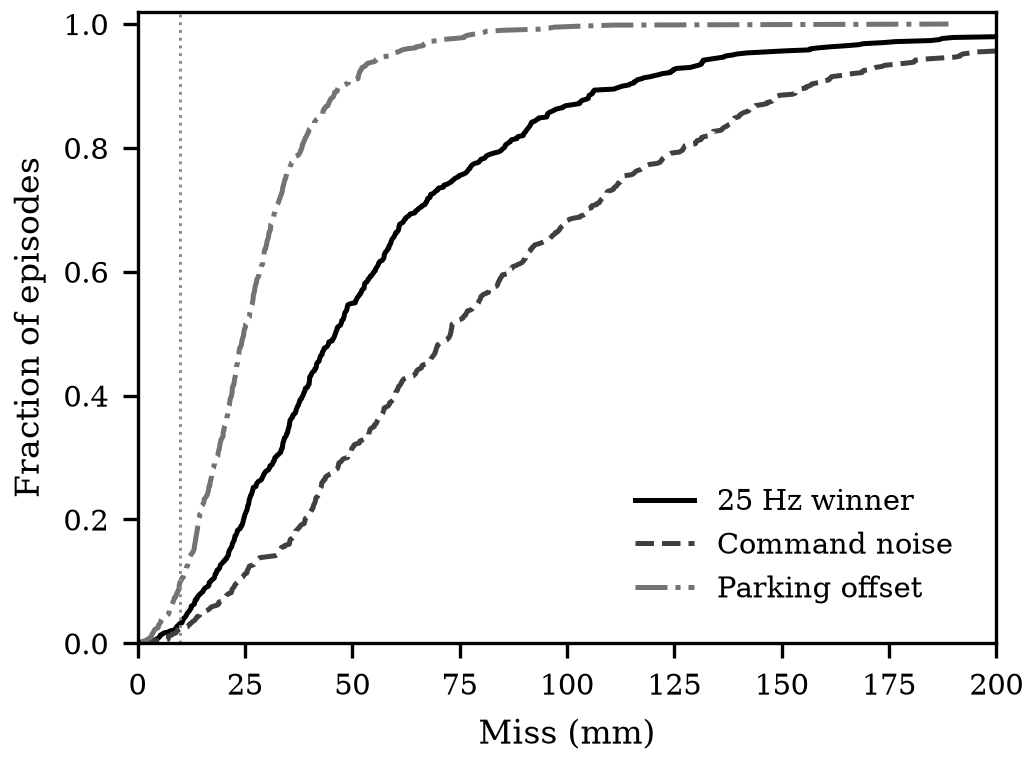
\includegraphics[width=\columnwidth]{rel_study_miss_ecdf.png}
\caption{Miss distribution for the three kept models, pooling three seeds and the 200 scenes. The dotted line is $10\,\mathrm{mm}$. The axis ends at $200\,\mathrm{mm}$. The winner's largest miss is $438\,\mathrm{mm}$ and the command-noise model's is $1042\,\mathrm{mm}$.}
\label{fig:miss}
\end{figure}

The winner's pooled median is $46\,\mathrm{mm}$, below its mean, because the tail reaches $438\,\mathrm{mm}$. Command noise moves the pooled median to $73\,\mathrm{mm}$. Parking offsets move it to $25\,\mathrm{mm}$, and no offset episode exceeds $189\,\mathrm{mm}$. As a description of that distribution, $55\%$ of winner episodes, $32\%$ of command-noise episodes and $91\%$ of offset episodes come within $50\,\mathrm{mm}$. The ranking criterion remains $10\,\mathrm{mm}$.

At the closest approach the winner's median absolute hand miss is $11\,\mathrm{mm}$ along the expert's route and $41\,\mathrm{mm}$ sideways. The base sits a median of $40\,\mathrm{mm}$ from the expert. The sideways coefficient is $-0.23$: the sideways hand error grows by more than the sideways parking error. The along-track coefficient is $0.62$. Figs.~\ref{fig:parkscatter}--\ref{fig:brake} use the same 600 episodes, three seeds on the 200 scenes. They show where that base stops in the expert's route frame, how far it sits off the expert path, and when the forward command brakes.

\begin{figure*}[t]
\centering
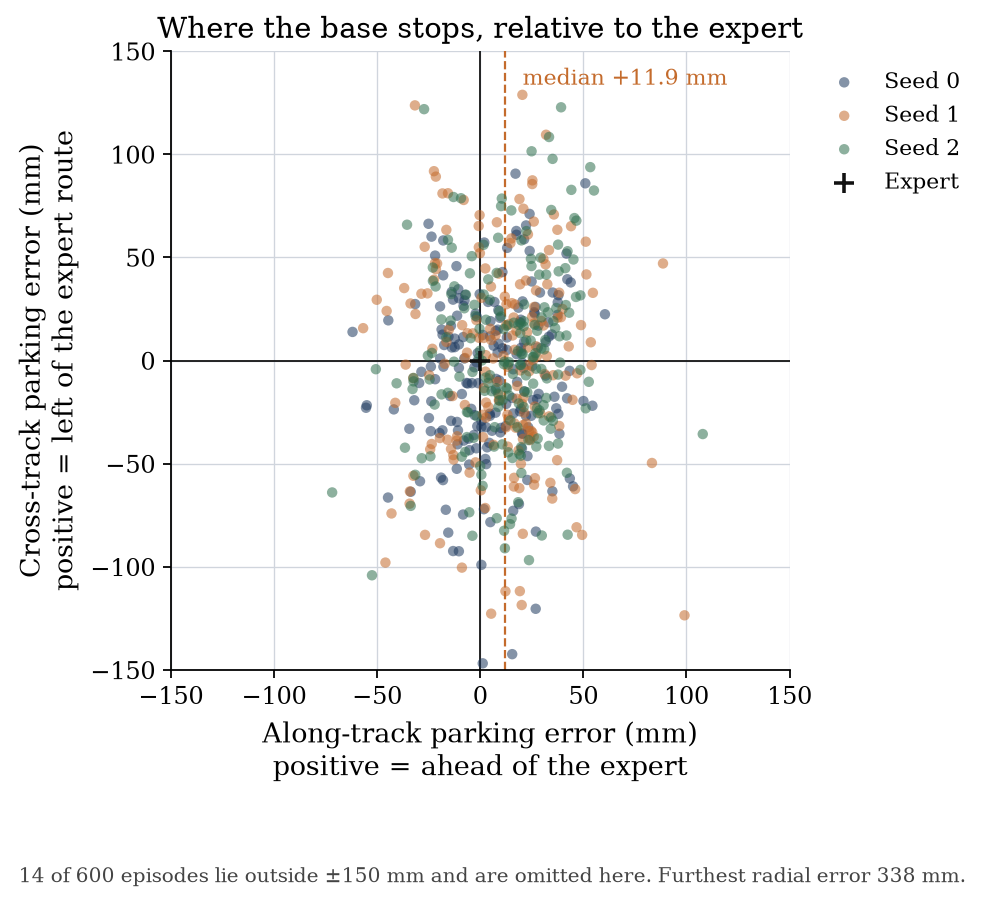
\includegraphics[width=\textwidth]{robotnik_arm/experiments/ablation/results/rel_study/plots/01_scatter.png}
\caption{Where the $25\,\mathrm{Hz}$ winner stops, relative to the expert, over 600 episodes. Positive along-track is ahead of the expert and positive cross-track is to the left of the route. The dashed line is the median along-track error, $+11.9\,\mathrm{mm}$. Fourteen episodes lie outside $\pm 150\,\mathrm{mm}$; the furthest radial error is $338\,\mathrm{mm}$.}
\label{fig:parkscatter}
\end{figure*}

\begin{figure*}[t]
\centering
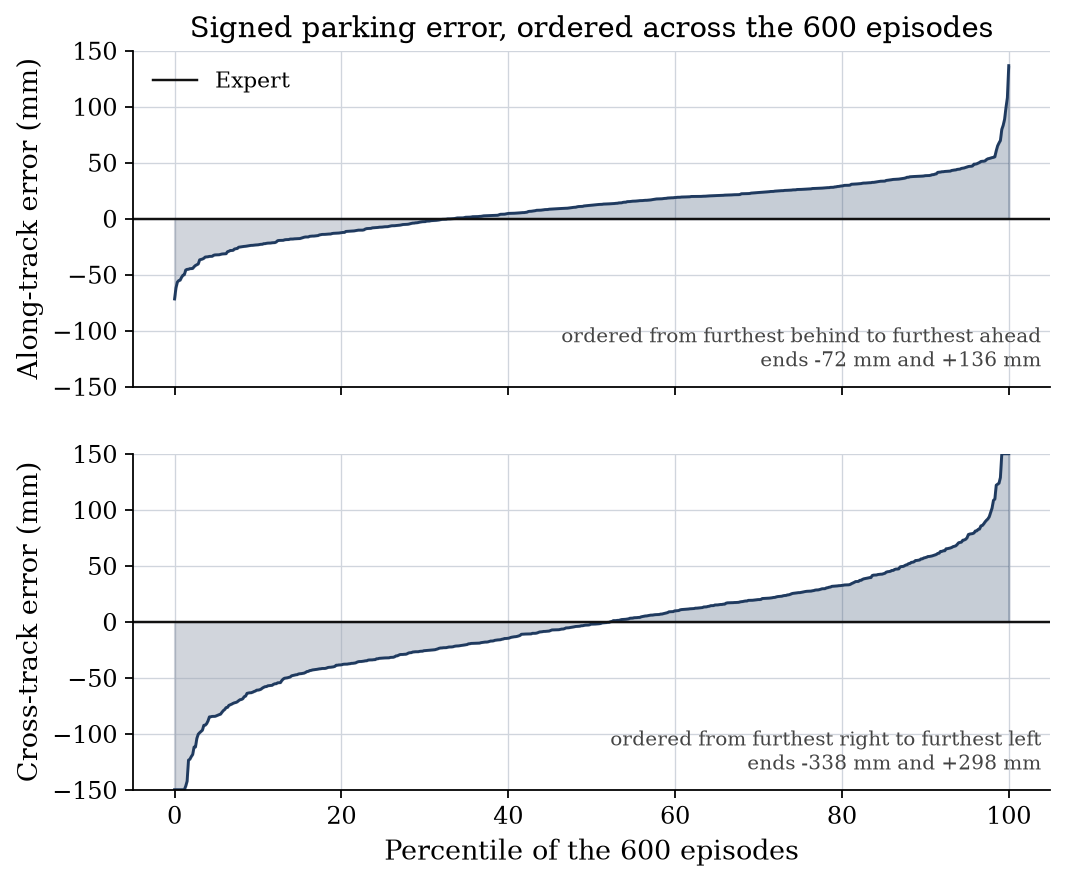
\includegraphics[width=0.72\textwidth]{robotnik_arm/experiments/ablation/results/rel_study/plots/04_ranked.png}
\caption{Signed parking error on the same 600 episodes. The upper panel is ordered from furthest behind to furthest ahead, and runs from $-72\,\mathrm{mm}$ to $+136\,\mathrm{mm}$. The lower panel is ordered from furthest right to furthest left, and runs from $-338\,\mathrm{mm}$ to $+298\,\mathrm{mm}$. Values outside $\pm 150\,\mathrm{mm}$ are clipped to the axis.}
\label{fig:parkranked}
\end{figure*}

\begin{figure*}[t]
\centering
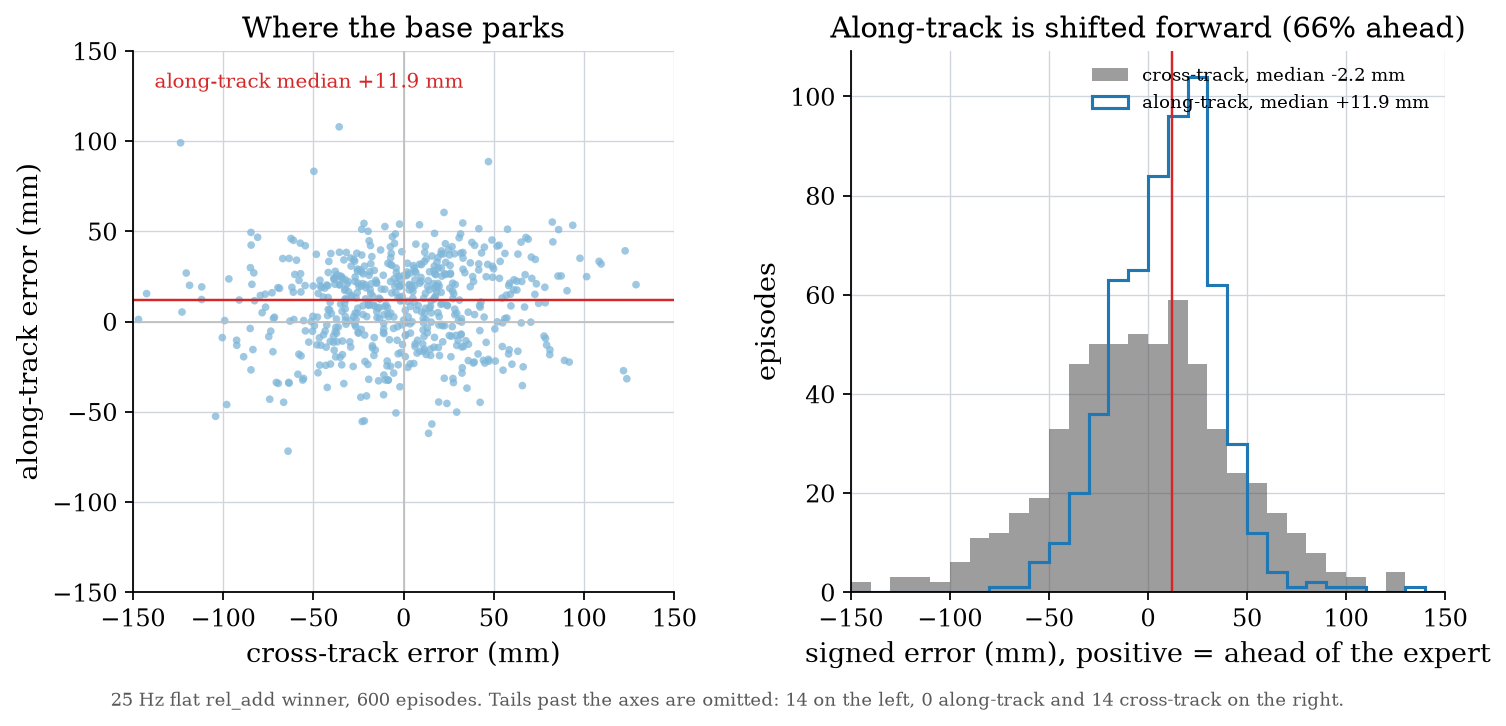
\includegraphics[width=\textwidth]{robotnik_arm/experiments/ablation/results/rel_study/plots/parking_bias.png}
\caption{Route-frame components of the same stops. The along-track median is $+11.9\,\mathrm{mm}$, and $66\%$ of episodes finish ahead of the expert. The cross-track median is $-2.2\,\mathrm{mm}$. The 14 episodes outside $\pm 150\,\mathrm{mm}$ are all cross-track outliers.}
\label{fig:parkbias}
\end{figure*}

\begin{figure*}[t]
\centering
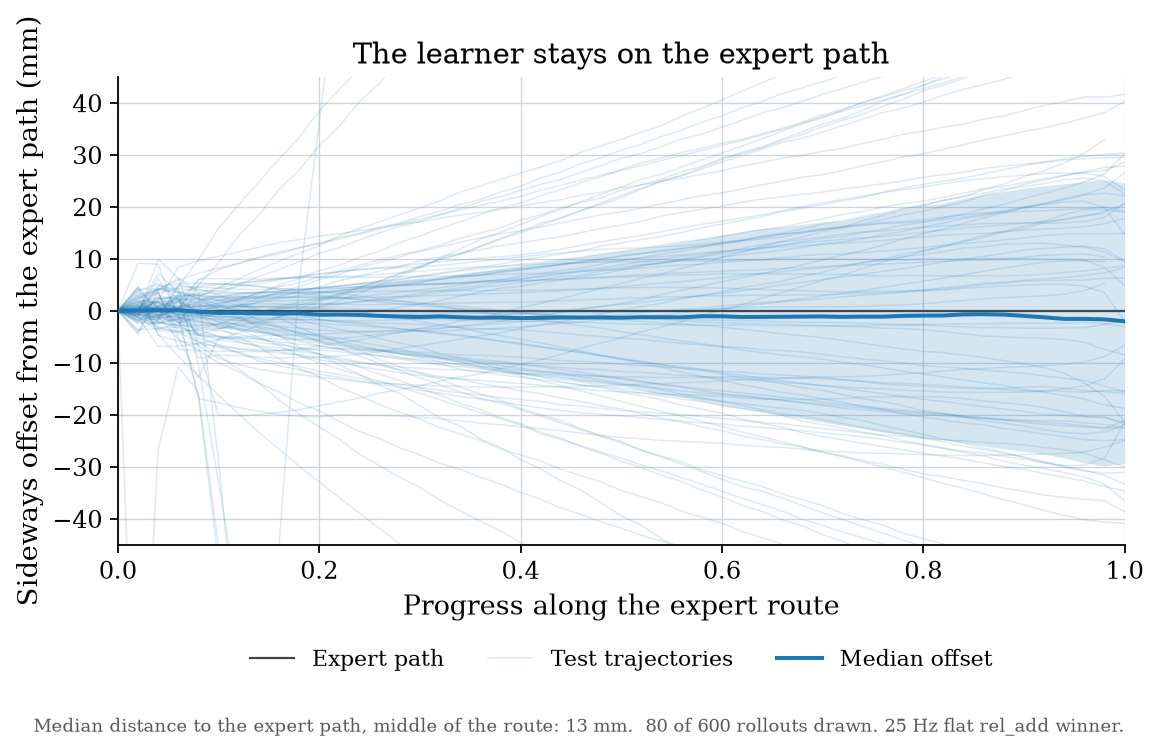
\includegraphics[width=0.78\textwidth]{robotnik_arm/experiments/ablation/results/rel_study/plots/path_adherence.png}
\caption{Sideways offset from the expert path against progress along the route, for the same 600 episodes. Eighty trajectories are drawn. The median distance to the path in the middle of the route is $13\,\mathrm{mm}$.}
\label{fig:path}
\end{figure*}

\begin{figure*}[t]
\centering
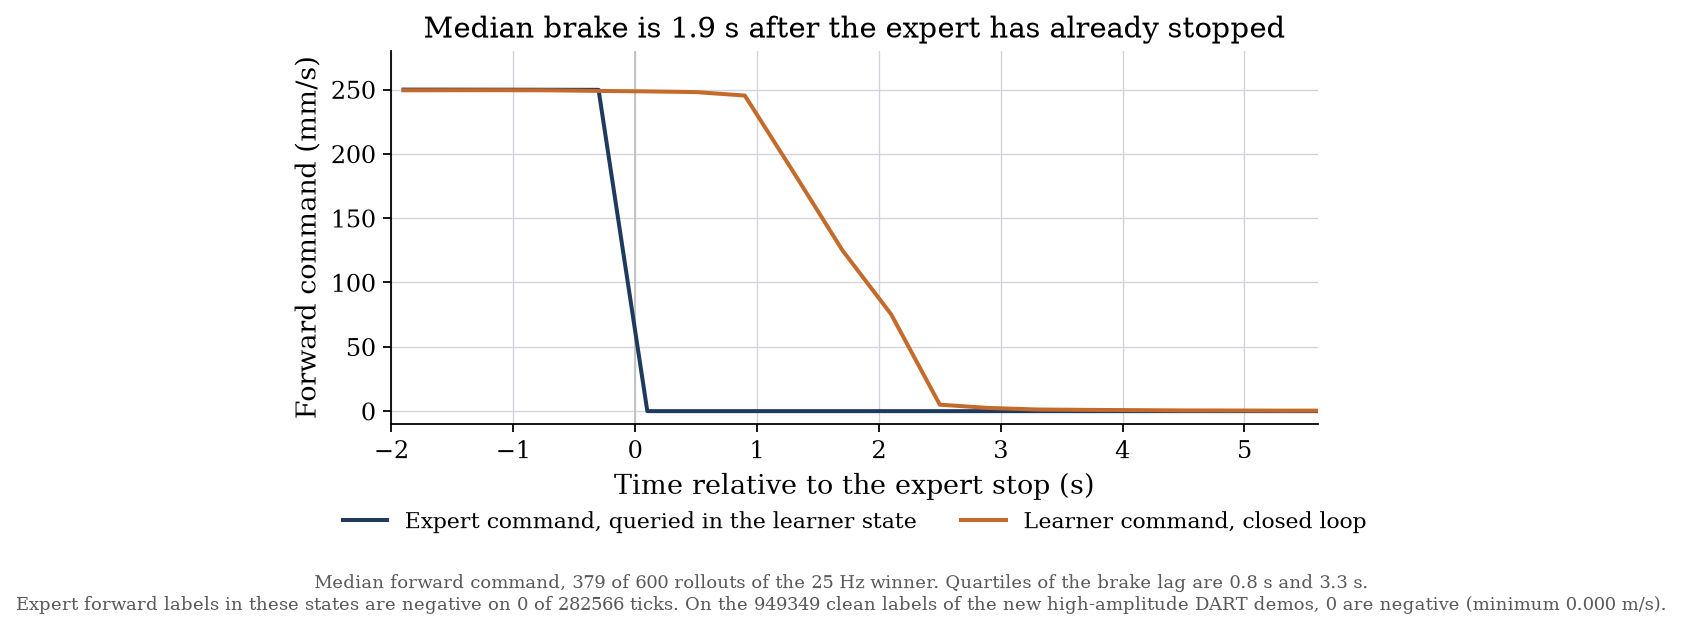
\includegraphics[width=0.78\textwidth]{robotnik_arm/experiments/ablation/results/rel_study/plots/01_brake_lag.png}
\caption{Median forward command of the $25\,\mathrm{Hz}$ winner, aligned to the expert stop. The expert curve is the command queried in the learner's closed-loop state and is not the command that was executed. On the 379 of 600 rollouts that come to a stop, the median brake is $1.9\,\mathrm{s}$ later. The quartiles are $0.8\,\mathrm{s}$ and $3.3\,\mathrm{s}$.}
\label{fig:brake}
\end{figure*}

The command noise was measured on 50 rollouts of this winner. It is an Ornstein--Uhlenbeck process on the executed command, with a standard deviation and a correlation time on each of the 18 channels. None of the correlation times was missing. The mean wheel standard deviation is $1.67\,\mathrm{rad/s}$, the mean arm-position standard deviation is $0.095\,\mathrm{rad}$, and the mean arm-velocity standard deviation is $0.031\,\mathrm{rad/s}$. The stored label is the clean expert command. Executed under that noise, the expert catches none of the $1{,}000$ added episodes and misses by $1133\,\mathrm{mm}$ on average. The policy trained on the combined set keeps the winner's along-track coefficient, $0.62$, and reaches a sideways coefficient of $0.33$. Its median absolute misses are $41\,\mathrm{mm}$ along the route, $33\,\mathrm{mm}$ sideways and $35\,\mathrm{mm}$ vertically, and the median base offset grows from $40\,\mathrm{mm}$ to $86\,\mathrm{mm}$. High-amplitude command noise raises the closed-loop miss.

The parking-offset policy uses the same added seeds. Its sideways coefficient is $1.00$ and its along-track coefficient is $0.45$. The median absolute sideways miss falls to $12\,\mathrm{mm}$. The along-track miss stays near $14\,\mathrm{mm}$, and the median base offset stays near $44\,\mathrm{mm}$. The hand corrects a sideways parking error. The along-track correction is lower than the winner's.

\subsection{Cost and Scope}
The $10\,\mathrm{Hz}$ network has $7.4\times 10^{5}$ parameters and a mean training time of $92\,\mathrm{s}$. The $25\,\mathrm{Hz}$ winner has $1.02\times 10^{6}$ parameters, because it predicts 50 steps rather than 20, and trains in $193\,\mathrm{s}$. The $50\,\mathrm{Hz}$ network predicts 100 steps, has $1.48\times 10^{6}$ parameters, and trains in $199\,\mathrm{s}$. The $10\,\mathrm{Hz}$ GRU has $8.7\times 10^{5}$ parameters and trains in $432\,\mathrm{s}$. The two $2{,}000$-episode retrains take $116\,\mathrm{s}$ and $119\,\mathrm{s}$. These are mean wall-clock times of the training process across the three seeds. Closed-loop inference latency was not measured.

The 200 scenes are a held-out seed list from the same generator as the training scenes. They are not a change of task. Observation noise, actuation latency and trajectories outside that generator were not measured. Every quoted mean includes the long tail. The $0.1\,\mathrm{s}$ chunk is the extreme case: its mean miss is above a metre because individual episodes miss by more than two.

\section{Discussion and Limitations}
\subsection{What the Evidence Supports}
The baseline analysis and the sweep agree on two of the three predictions that cleared their thresholds. A higher rate lowers the miss, and a half-second chunk increases it. They disagree on the horizon. Open-loop error grows by a factor of ten along the chunk, which predicted that the shorter prediction would be the better one. With execution held at $1\,\mathrm{s}$, the closed-loop sweep ranks the $5\,\mathrm{s}$ prediction ahead of the $1\,\mathrm{s}$ prediction. The execution-window measurement stayed below its threshold, and cutting the window to $0.5\,\mathrm{s}$ made the miss worse. History stayed below its threshold, and no history level moves the $10\,\mathrm{Hz}$ miss by more than a few millimetres. Base-frame features are in every model, so their contribution is not a measured step.

The three kept models support a specific account of the two extensions. Parking offsets lower the miss and bring the sideways correction coefficient to one. High-amplitude command noise raises the miss, leaves the along-track coefficient where the winner had it, and does not reach that sideways correction. The offset model's along-track coefficient is lower than the winner's, so the gain is the sideways component of the hand error, which was the winner's larger horizontal component.

\subsection{Limits of the Perturbation Comparison}
Half of the original $1{,}000$ episodes already carry low-amplitude torque noise. The later command-noise set is a different perturbation: Ornstein--Uhlenbeck noise on the executed command, sized to this winner's own error, with the clean command kept as the label. The parking set moves the goal and leaves the commands clean. The two extensions match each other in scene seeds and in the number of episodes added. Each one also changes the training set from $1{,}000$ episodes to $2{,}000$, so a comparison against the winner mixes the perturbation with the extra data. The comparison between the two extensions does not. The noise matches per-channel variance and correlation time. It does not shift the parking position, and the compensation table is the evidence that the offset demonstrations do something the noise does not.

\subsection{Validity, Reproducibility and Remaining Gaps}
The factor sweeps change one setting at a time, and only the combination stage changes families together. Holding a chunk's duration fixed in seconds means a higher policy rate also predicts and executes more steps, so the rate comparison is not a change of clock alone. Inputs are noise-free simulated state. There is no hardware trial and no grasp. Robustness to observation noise and performance on trajectories outside the training distribution have not been measured. The 200 evaluation scenes are the development benchmark used to rank the sweep. A configuration chosen on those scenes has not been confirmed on a list that was withheld from the ranking.
\subsection{Future Work}
A scene list frozen before the ranking, a larger set of training seeds, observation noise, and a hardware trial would test whether the order in Table~\ref{tab:sweep} survives. The hand-off probe, which misses by only a few millimetres, is the wrong place to look for the $113\,\mathrm{mm}$ closed-loop failure. That diagnosis has to cover the episode from the start. None of these tests is assigned an expected gain.

\section{Conclusion}
Policy rate is the factor the baseline analysis indicated and the ranking confirms. The selected controller runs at $25\,\mathrm{Hz}$, predicts $2\,\mathrm{s}$, executes $1\,\mathrm{s}$, and uses the current frame. On the 200 development scenes its mean miss is $59\,\mathrm{mm}$ and $3.2\%$ of episodes come within $10\,\mathrm{mm}$, against $113\,\mathrm{mm}$ and $0.7\%$ for the $10\,\mathrm{Hz}$ baseline. Fifty hertz has the higher catch rate. The seed intervals overlap and its miss is not lower, so it is not the winner. History, a shorter prediction, and a shorter execution window do not improve the baseline. A half-second chunk makes the miss several times larger. High-amplitude command noise matched to the winner raises the mean miss to $90\,\mathrm{mm}$. Parking-offset demonstrations lower it to $28\,\mathrm{mm}$ and bring the sideways correction to one. The along-track correction does not improve. The study uses simulated state, a flat network, and no grasp. Observation noise, trajectories outside the training generator, and hardware remain untested.

% Approx. 0.5 page reserved for the references below.
\begin{thebibliography}{1}
\bibitem{pomerleau1991}
D.~A. Pomerleau, ``Efficient training of artificial neural networks for autonomous navigation,'' \emph{Neural Comput.}, vol.~3, no.~1, pp.~88--97, 1991.
\bibitem{ross2011}
S.~Ross, G.~J. Gordon, and J.~A. Bagnell, ``A reduction of imitation learning and structured prediction to no-regret online learning,'' in \emph{Proc. 14th Int. Conf. Artif. Intell. Statist.}, 2011, pp.~627--635.
\bibitem{laskey2017}
M.~Laskey, J.~Lee, R.~Fox, A.~Dragan, and K.~Goldberg, ``{DART}: Noise injection for robust imitation learning,'' in \emph{Proc. 1st Conf. Robot Learn.}, 2017, pp.~143--156.
\bibitem{pybullet}
E.~Coumans and Y.~Bai, ``PyBullet, a Python module for physics simulation for games, robotics and machine learning,'' 2016. [Online]. Available: \url{http://pybullet.org}
\bibitem{pinocchio}
J.~Carpentier \emph{et al.}, ``The {P}inocchio {C}++ library: A fast and flexible implementation of rigid body dynamics algorithms and their analytical derivatives,'' in \emph{Proc. IEEE/SICE Int. Symp. Syst. Integr.}, 2019, pp.~614--619.
\end{thebibliography}

% Separate statement, up to one additional page under the assignment brief.
% Keep outside the six-page technical-report budget.
\clearpage
\section*{Contribution Statement}
% BLANK: group members must supply their actual contributions.

\end{document}
